\newpage
\section{RESULTADOS COMPUTACIONAIS, VERIFICAÇÃO DA PINN E CONTROLE ATIVO TEMS}
\label{cap:resultados}

Este capítulo apresenta os resultados numéricos verificados da planta térmica de referência no vácuo (Marco~3), a auditoria completa do Modelo Substituto Preditivo Baseado em Física (PINN, Marco~4) — incluindo ablações, validação independente em $500$ casos \textit{Latin Hypercube}, robustez multi-semente, comparação contra modelos concentrados RC e desempenho do estimador de gradiente — e a arquitetura experimental do controlador ativo TEMS/DVFS em malha fechada (Marco~5). Ressalta-se que todos os resultados aqui reportados são estritamente \textit{in silico} (verificação contra o solucionador de volumes finitos, sem ensaio em câmara termo-vácuo ou emulador HIL).

% ==============================================================================
\subsection{Verificação da Planta Térmica de Referência no Vácuo (Marco 3)}
\label{sec:resultados_marco3}

O solucionador de volumes finitos (\texttt{modelo\_termico.py}, discretização espacial com $N=160$ nós e integração temporal por Crank-Nicolson com partida de Rannacher e resolução de Newton-Raphson) foi verificado por uma suíte automatizada de $12$ testes unitários e de conferência cruzada (\texttt{12 passed}), confirmando:
\begin{itemize}
    \item \textbf{Ordem de convergência verificada:} taxa espacial e temporal medida em $2{,}00$ contra soluções analíticas de referência (aleta linear, integral primeira da aleta radiante não linear e resfriamento radiativo concentrado).
    \item \textbf{Conservação estrita de energia:} resíduo relativo do balanço global de energia de $3{,}13 \times 10^{-13}$ em regime periódico e $\le 1{,}73 \times 10^{-6}$ em janelas transientes de $300\text{ s}$.
    \item \textbf{Dimensionamento do radiador:} para sustentar a potência computacional máxima energeticamente viável no sol ($P_{TI,sol,sust} = 38{,}18\text{ kW}$, com $18{,}0\text{ kW}$ no eclipse e banco BESS Saft VES~16 em $19\text{P}108\text{S}$, $2.052$ células, $236{,}0\text{ kg}$), sob revestimento Z-93 EOL conservador ($\alpha_s = 0{,}36$, $\varepsilon = 0{,}90$), a área de planta requerida para manter $T_j \le 80^\circ\text{C}$ é $A_{pl} = 49{,}90\text{ m}^2$ ($A_{emit} = 99{,}80\text{ m}^2$).
\end{itemize}

Em regime periódico orbital (LTAN $18\text{h}00$, $\beta = 58{,}374^\circ$, eclipse de $1.105{,}39\text{ s}$), o cenário sem controle de carga (\textbf{S0}, $1.410\text{ MHz}$ / $40\text{ kW}$ contínuos) eleva a temperatura de junção a $T_{j,\max} = 86{,}67^\circ\text{C}$ (violando o limite de $80^\circ\text{C}$ em $6{,}67\text{ K}$ e esgotando o BESS), enquanto o despacho estático sustentável (\textbf{S1}) mantém $T_{j,\max} = 78{,}52^\circ\text{C}$, resultando em uma \textbf{folga térmica nominal de apenas $1{,}48\text{ K}$} frente ao teto de $80^\circ\text{C}$.

% ==============================================================================
\subsection{Verificação e Auditoria Robusta do Preditor PINN (Marco 4)}
\label{sec:resultados_marco4}

A suíte automatizada da PINN versão 2 (\texttt{modelo\_pinn.py}, PyTorch puro, $26.178$ parâmetros, sem termo de dados supervisionados) passou integralmente em CPU livre (\texttt{14 passed}). A evolução das ablações de treinamento — partindo da versão baseline até a inclusão de condição inicial exata por construção (\texttt{--hard\_ic}), normalização das perdas em kelvin equivalente, amostragem correlacionada ($T_{j,0} - T_{raiz,0} \in [5,\; 40]\text{ K}$) e refinamento quasi-Newton (\textbf{L-BFGS}, $50$ passos sobre lote fixo de colocação) — está consolidada na Tabela~\ref{tab:pinn_ablacoes} e ilustrada na Figura~\ref{fig:pinn_ablacoes}.

\begin{table}[htbp]
\centering
\small
\caption{Evolução das ablações de treinamento da PINN pura (zero dados do solver) avaliadas nos $10$ casos dentro do domínio de treino v2.}
\label{tab:pinn_ablacoes}
\begin{tabularx}{\textwidth}{>{\raggedright\arraybackslash}Xcccccc}
\toprule
\textbf{Modelo / Execução} & \textbf{Pior erro ($^\circ$C)} & \textbf{Mediana ($^\circ$C)} & \textbf{Casos $\le 0{,}5^\circ$C} & \textbf{Pior subest. pico ($^\circ$C)} & \textbf{RMS $L_{pde}$ / $L_{bc}$ (K)} \\
\midrule
Base (v1, 6k Adam) & $9{,}95$* & $\approx 4{,}0$* & $0/23$* & $-9{,}95$* & — \\
E1 (\texttt{--hard\_ic}, 6k) & $2{,}97$* & $1{,}81$* & $1/23$* & $-2{,}68$* & — \\
E2 (E1 + $w_{bc}=25$, 6k) & $2{,}47$* & $1{,}24$* & $5/23$* & $-2{,}32$* & — \\
E3 (E2, 20k Adam) & $1{,}53$ & $0{,}56$ & $5/10$ & $-1{,}13$ & $1{,}34$ / $0{,}33$ \\
V2a (K-eq, indep, 20k) & $1{,}79$ & $0{,}44$ & $6/10$ & $-1{,}30$ & $0{,}69$ / $0{,}87$ \\
V2b (K-eq, corr, 20k) & $1{,}46$ & $0{,}55$ & $4/10$ & $-1{,}09$ & $0{,}78$ / $0{,}95$ \\
\textbf{V2c (V2b + 50 L-BFGS)} & \textbf{$0{,}47$} & \textbf{$0{,}27$} & \textbf{$10/10$} & \textbf{$-0{,}41$} & $1{,}76$ / $0{,}30$ \\
\bottomrule
\end{tabularx}
\\[2pt]
{\footnotesize *Métricas sobre todos os $23$ casos na régua v1; a partir de E3, valores reportados no domínio de treino v2 ($n=10$).}
\end{table}

\begin{figure}[htbp]
    \centering
    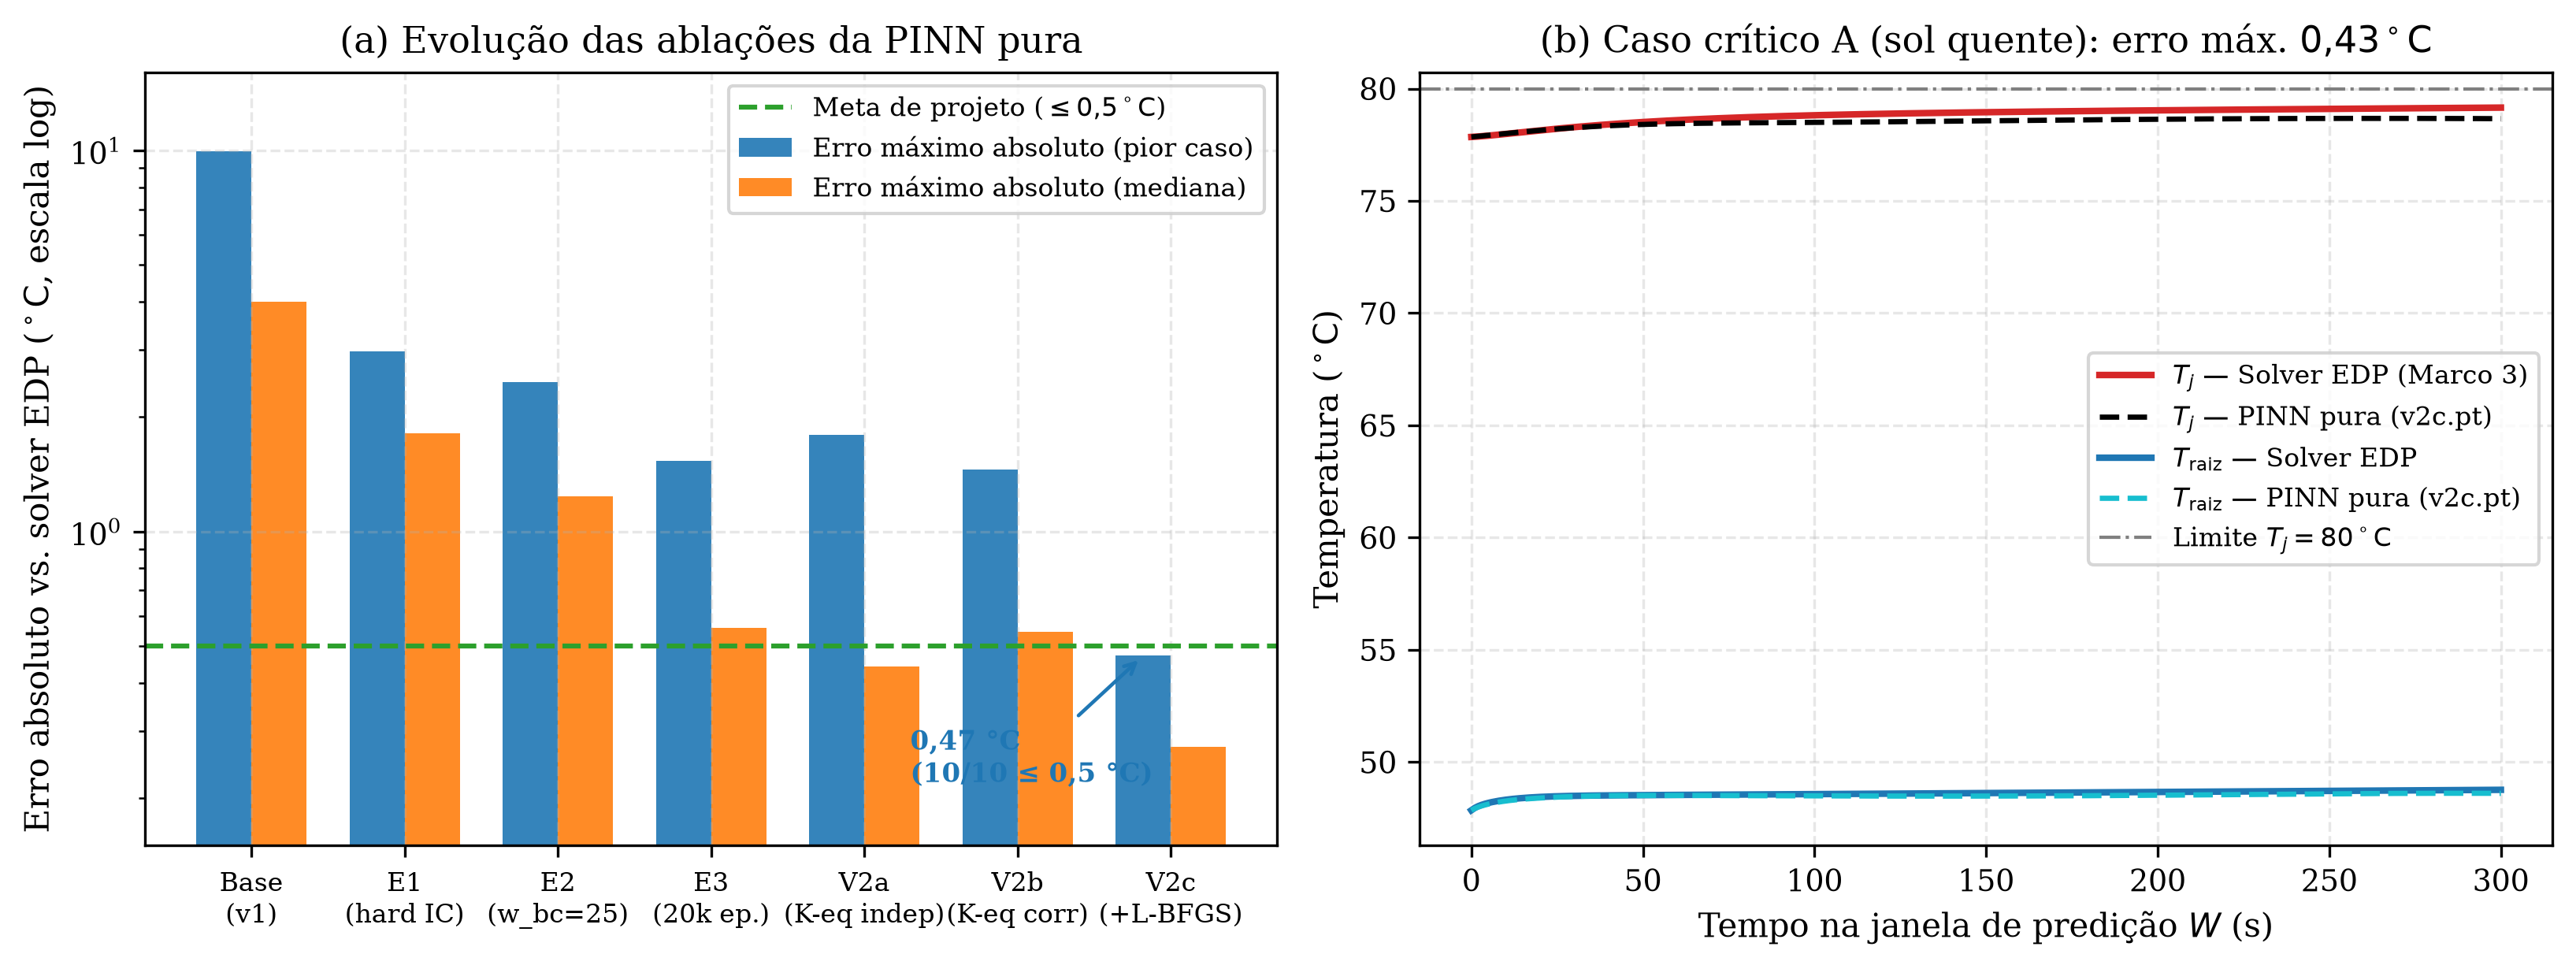
\includegraphics[width=0.98\textwidth]{figuras/fig_4_1_pinn_ablacoes_e_validacao.png}
    \caption{Verificação da PINN pura (\texttt{v2c.pt}): (a) redução do erro absoluto ao longo das ablações de treinamento; (b) aderência das trajetórias de $T_j(t)$ e $T_{raiz}(t)$ frente ao solver EDP no caso crítico A (sol quente, erro máximo $0{,}43^\circ\text{C}$, resíduo de energia $-0{,}29\%$).}
    \label{fig:pinn_ablacoes}
\end{figure}

\subsubsection{Auditoria Independente em 500 Casos LHS, Degradação OOD e Concorrentes RC}

Como o conjunto de avaliação padrão contém apenas $10$ casos dentro do domínio, realizou-se uma auditoria independente por amostragem \textit{Latin Hypercube} (\texttt{auditoria\_marco4\_robusta.py}) com $300$ casos no interior do domínio de treino ($d_{\mathrm{box}} = 0$) e $200$ casos fora do domínio ($d_{\mathrm{box}} > 0$), comparando o checkpoint congelado \texttt{v2c.pt} contra dois concorrentes físicos concentrados sem ajuste empírico: um modelo RC clássico de $2$ nós (junção + radiador único) e um modelo RC físico de $3$ nós (junção + coletor + aleta média com condutância analítica $G_{fin} = \ell k \delta / (L/3)$). Os resultados são apresentados na Tabela~\ref{tab:auditoria_500_rc} e na Figura~\ref{fig:pinn_500_ood_rc}.

\begin{table}[htbp]
\centering
\small
\caption{Auditoria independente em $500$ casos LHS ($300$ no domínio + $200$ OOD), comparação contra modelos RC físicos e benchmark de latência em CPU (1 thread, $16$ instantes de saída).}
\label{tab:auditoria_500_rc}
\begin{tabularx}{\textwidth}{>{\raggedright\arraybackslash}Xccccc}
\toprule
\textbf{Modelo / Região (LHS)} & \textbf{Mediana ($^\circ$C)} & \textbf{p95 ($^\circ$C)} & \textbf{Pior ($^\circ$C)} & \textbf{Pior subest. ($^\circ$C)} & \textbf{Latência média / p99} \\
\midrule
\textbf{PINN \texttt{v2c.pt} ($d=0$, $n=300$)} & $0{,}206$ & $0{,}664$ & $0{,}904$ & $-0{,}720$ & \textbf{$0{,}70$ / $1{,}57\text{ ms}$} \\
PINN OOD ($0 < d \le 0{,}15$, $n=31$) & $0{,}337$ & $0{,}854$ & $0{,}931$ & $-0{,}317$ & — \\
PINN OOD ($0{,}15 < d \le 0{,}35$, $n=42$) & $0{,}629$ & $1{,}725$ & $2{,}179$ & $-0{,}444$ & — \\
PINN OOD ($d > 0{,}35$, $n=127$) & $4{,}520$ & $19{,}70$ & $28{,}09$ & $-0{,}515$ & — \\
RC 2 nós (física pura, $n=300$) & $2{,}690$ & $4{,}085$ & $5{,}117$ & $-5{,}117$ & — \\
RC 3 nós (Radau, $n=300$) & $0{,}123$ & $0{,}282$ & $0{,}338$ & $-0{,}258$ & $6{,}95$ / $10{,}92\text{ ms}$ \\
RC 3 nós (Euler impl. 16 passos) & — & — & — & — & $1{,}49$ / $4{,}09\text{ ms}$ \\
Solver EDP ($N=160$, $\Delta t=1\text{ s}$) & \textit{ref.} & \textit{ref.} & \textit{ref.} & $0{,}0$ & $124{,}54$ / $168{,}06\text{ ms}$ \\
\bottomrule
\end{tabularx}
\end{table}

\begin{figure}[htbp]
    \centering
    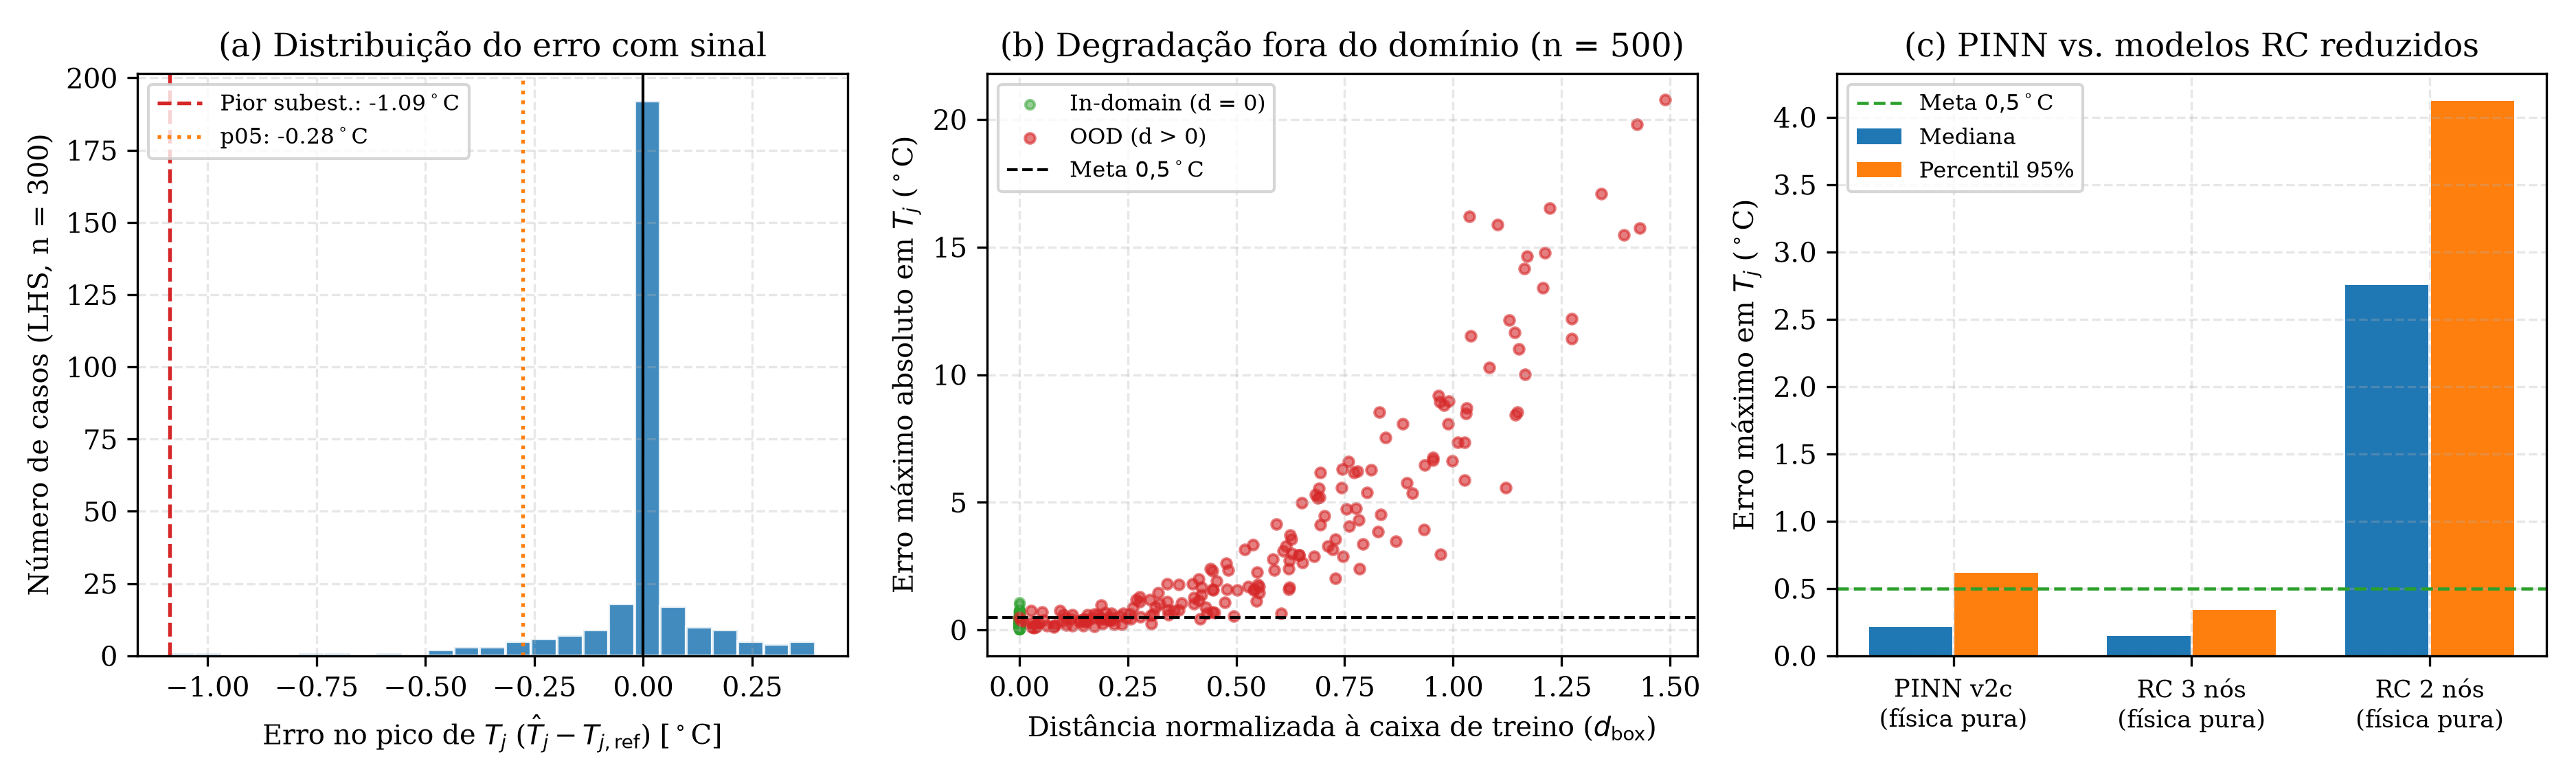
\includegraphics[width=0.98\textwidth]{figuras/fig_4_2_pinn_500casos_ood_rc.png}
    \caption{Auditoria robusta do Marco 4: (a) distribuição do erro com sinal no pico de $T_j$ ($n=300$ no domínio); (b) degradação fora do domínio em função de $d_{\mathrm{box}}$ ($n=500$); (c) comparação direta entre PINN \texttt{v2c.pt} e modelos concentrados RC de 2 e 3 nós.}
    \label{fig:pinn_500_ood_rc}
\end{figure}

Os resultados impõem três conclusões transparentes de rigor científico:
\begin{enumerate}
    \item \textbf{Atendimento parcial da meta de pior caso absoluto:} embora $85{,}3\%$ ($256/300$) dos casos no domínio fiquem em $\le 0{,}5^\circ\text{C}$ (mediana de $0{,}206^\circ\text{C}$ e viés médio quase nulo de $+0{,}008^\circ\text{C}$), o percentil $95\%$ atinge $0{,}664^\circ\text{C}$, o pior caso atinge $0{,}904^\circ\text{C}$ e a pior subestimação do pico é $-0{,}720^\circ\text{C}$ (adotada como $m_{pred} = 0{,}72\text{ K}$ no projeto de margem do controlador).
    \item \textbf{Justificativa honesta frente ao RC3:} a PINN supera amplamente o modelo RC clássico de $2$ nós ($13\times$ menor erro mediano), mas o modelo RC físico de $3$ nós é mais exato neste caso 1D concentrável (mediana $0{,}123^\circ\text{C}$, pior $0{,}338^\circ\text{C}$). A vantagem objetiva da PINN reside na \textbf{velocidade de inferência não-iterativa} ($0{,}70\text{ ms}$ em 1 thread: $177{,}3\times$ mais rápida que o solver EDP $N=160$, $10\times$ mais rápida que RC3-Radau e $2{,}1\times$ mais rápida que RC3-Euler implícito), na diferenciabilidade nativa e na representação contínua do campo $T(x,t)$. Por esse motivo, o RC3 é incluído como preditor concorrente direto no Marco~5.
    \item \textbf{Necessidade da barreira de domínio:} fora do domínio de treino ($d_{\mathrm{box}} > 0{,}35$), o erro da PINN degrada severamente (até $28{,}09^\circ\text{C}$), tornando mandatória a camada de supervisão de domínio com \textit{fallback} seguro no controlador.
\end{enumerate}

\subsubsection{Robustez Multi-Semente, Reamostragem do L-BFGS e Estimador de $\Delta_{ponta}$}

Para descartar dependência de inicialização aleatória, executou-se uma campanha independente de \textbf{5 sementes} (\texttt{seed=0..4}, $20.000$ passos Adam + $50$ passos L-BFGS em GPU NVIDIA L4/T4, \texttt{saida\_marco4\_colab\_5seeds\_resumo.json}):
\begin{itemize}
    \item \textbf{Estabilidade entre sementes ($n=10$ no domínio):} mediana de $0{,}294 \pm 0{,}026^\circ\text{C}$ (variabilidade inferior a $0{,}03^\circ\text{C}$), pior caso de $0{,}624 \pm 0{,}164^\circ\text{C}$ (faixa de $0{,}465$ a $0{,}871^\circ\text{C}$) e pior subestimação do pico entre todas as cinco sementes de $-0{,}694^\circ\text{C}$ (consistente com os $-0{,}720^\circ\text{C}$ da auditoria LHS).
    \item \textbf{Diagnóstico do L-BFGS:} a reamostragem do lote fixo de colocação a partir de \texttt{v2b.pt} demonstrou que dobrar o tamanho do lote de $n_{s,\text{L-BFGS}} = 96$ para $192$ reduz o resíduo de validação da EDP ($L_{pde,\text{val}}$) em $2{,}5\times$ (de $1{,}85\text{ K}$ para $0{,}73\text{ K}$), confirmando que o resíduo elevado em pontos não vistos decorre do tamanho do lote fixo e não de falha estrutural da formulação.
    \item \textbf{Desempenho do estimador de $\Delta_{ponta}$:} sobre $20$ casos novos no domínio ($w_{obs} = 60\text{ s}$), o estimador por mínimos quadrados ponderados reduz o erro RMS em $T_j(300\text{ s})$ de $1{,}195\text{ K}$ (sem estimador) para $0{,}274\text{ K}$ sob ruído e viés de $T_j$ ($\pm 1{,}5\text{ K}$) e $0{,}265\text{ K}$ sob viés de RTD ($\pm 0{,}25\text{ K}$), atingindo o piso da própria PINN ($0{,}286\text{ K}$ com $\Delta_{ponta}$ exato), com latência média de $2{,}19\text{ ms}$ ($p99 = 4{,}26\text{ ms}$).
\end{itemize}

% ==============================================================================
\subsection{Controle Ativo TEMS/DVFS em Malha Fechada (Marco 5)}
\label{sec:resultados_marco5}

A integração em malha fechada encontra-se implementada e verificada em \texttt{contrato\_parametros.py}, \texttt{marco5\_tems.py} e \texttt{test\_marco5.py} (\texttt{14 passed in 10.12s} com PyTorch e verificação automática de \texttt{SHA256} do checkpoint congelado \texttt{v2c.pt}), adotando controle preditivo supervisório com \textit{move blocking} ($f$ comum em $[300,\; 1.410]\text{ MHz}$, período de controle $\Delta t_{ctrl} = 60\text{ s}$, horizonte $W = 300\text{ s}$ alinhado às quebras de eclipse), barreira de domínio OOD e supervisor energético comum de órbita completa.

Os critérios pré-registrados de avaliação (P1 a P5) comparam cinco arquiteturas: \textbf{S0} (sem controle), \textbf{S1} (estático offline), \textbf{R} (reativo PI sintonizado em sementes de calibração disjuntas das de teste), \textbf{TEMS+RC3} (preditor físico concorrente), \textbf{TEMS+PINN} (proposta) e \textbf{Oráculo} (solver EDP). A verificação preliminar de integração em $3$ órbitas nominais (\texttt{m5\_nominal.json}, sensor sem calibração, semente $0$) já confirmou ausência de violações térmicas e de $SoC$ tanto para \texttt{TEMS\_PINN} ($T_{j,\max} = 78{,}33^\circ\text{C}$, $SoC_{\min} = 0{,}700$, vazão $0{,}875$, resíduo de energia $1{,}84 \times 10^{-12}$) quanto para \texttt{TEMS\_RC3} ($78{,}28^\circ\text{C}$, vazão $0{,}874$), com \textbf{decisão completa $4{,}2\times$ mais rápida na PINN} ($14{,}30\text{ ms}$ média / $34{,}56\text{ ms}$ p99 contra $59{,}63\text{ ms}$ / $142{,}53\text{ ms}$ do RC3), ao passo que \textbf{S0} colapsou ($86{,}66^\circ\text{C}$, $SoC = 0$).

\textit{Nota de encerramento experimental:} os resultados definitivos da campanha completa do Marco~5 — abrangendo $6$ órbitas em regime periódico, sintonia justa do controlador reativo (\texttt{R\_SINT}) em sementes disjuntas, rajadas de carga, perturbações paramétricas ($\varepsilon$, $R_{int}$, $C_{mod}$), quantização NVML, fronteira de Pareto em $m_T \in \{0,\; 0{,}5,\; 1,\; 2,\; 3\}\text{ K}$ e cenários OOD — serão consolidados nesta seção imediatamente após a execução da suíte completa.
